% 115 120
\documentclass[12pt,a4paper]{amsart}
\usepackage[slovene]{babel}
\usepackage[utf8]{inputenc}
\usepackage{amsmath,amssymb,amsfonts}
\usepackage{url}
\usepackage[dvipsnames,usenames]{color}
\usepackage{graphicx} 


\begin{document}
\title{Grafitti Conjecturre 194}
\author{Martin Praček, Mela Malej}
\maketitle
Za predmet Finančni praktikum v študijskem letu $2018/19$ Martin Praček in Mela Malej dobila nalogo predstaviti problem Grafittijeve konjekuture $194$. \\\\
\section{Predstavitev problema}
Grafittijeva konjektura 194 nam zastavi vprašanje iz teorije grafov.Zanima nas, ali za vsak preprost, povezan graf, ki zadošča pogoju $$ \alpha(G) \leq 1 + \lambda_{avg}(G)$$, velja, da obstaja hamiltonska pot. Gre za računalniško generirano trditev, pri kateri nas zanima, ali lahko najdemo protiprimer.\\
\section{Pogoji našega problema}
Naš pogoj je torej $ \alpha(G) \leq 1 + \lambda_{avg}(G),$
kjer je $G$ naš graf, $\alpha(G)$ je neodvistnostno število, $\lambda_{avg}$ pa je povprečna lokalna neodvistnost grafa.\\
\textbf{Neodvistnostno število grafa} $\alpha(G)$ nam pove moč največje množice, ki vsebuje  vozlišča grafa $G$, od katerih nobeni dve niste sosednji.\\
\textbf{Lokalna neodvistnost grafa} $\lambda(G, v)$ nam pove neodvistnostno število podgrafa $Gv$ grafa $G$, kjer je $Gv$ definiran na sosedih vozlišča $v$. $\lambda_{avg}(G)$ nam pove povprečno lokalno neodvistnost.\\
Ves čas zahtevamo, da je graf \textbf{preprost in povezan}. Ta zahteva pomeni, da ne obstaja vozlišče, ki ne bi bilo sosednje vsaj enemu drugemu vozlišču, poleg tega pa med dvema povezavama obstaja kvečjemu ena povezava in ne obstaja  povezave od vozlišča $v$ do vozlišča $v$, kar pomeni da ne obstajajo zanke na enem vozlišču.\\
 
\begin{figure}[h]
	\centering
	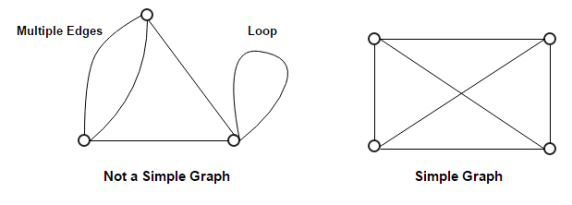
\includegraphics[scale=1]{slike/graf1}
	\caption{$http://mathworld.wolfram.com/images/eps-gif/SimpleGraph_950.gif$}
\end{figure}
Graf ima \textbf{hamiltonsko pot}, če obstajata dve vozlišči, ki ju povezuje pot, ki natančno enkrat obišče vsako vozlišče grafa.\\
\ \\
Najina naloga je torej na dovolj velikem vzorcu grafov pokazati da to velja, ali pa dobiti protiprimer, ki bo dokazal da to ne drži.\\
\section{Dosedanje delo}
Do sedaj sva začela s pisanjem kode, ki bo preverjala majhne grafe, torej do približno $30$ vozlišč. Za tako ločnico sva se odločila zaradi nekaj NP-težkih problemov, s katerimi morava v najini seminarski nalogi delati.  
\section{Prihodnje delo}
\end{document}